\section{Results of verification}
This section will quickly summarize the results of chapter \ref{chapter:analysis}.


\subsection{The FE scheme}
Although not all of the results from verification of the FE scheme are perfect, the results from testing the exact numerical solution are really good. 
The numerical exact solution test is a verification of the implementation of the FE scheme. 
A successful test indicates that the scheme is correct and will solve the diffusion equation to the expected accuracy. 
When the convergence tests for the FE scheme could be better it is most likely due to other effects like not being able to make the error from the spatial derivative sufficiently dominant. 
The result of verifying the FE scheme is that it is deemed correctly implemented within the limits of the applied tests.

\subsection{The BE scheme and the block tridiagonal solver}
Most of the tests done on the BE scheme are close to perfect. 
Only when testing the scheme versus the numerical exact solution are the results slightly off. 
Though the numerical exact solution test is expected to give an error close to machine precision the results are five orders of magnitude larger than machine precision. 
On the other hand, the error term is also eight orders of magnitude smaller than the time step and there are a lot of possible round off errors in the inverted coefficient matrix which might accumulate. \\
Effectively, testing the convergence rate also verifies the assembly of the coefficient matrix while testing against the numerical exact solution verifies that the block tridiagonal solver works properly.\\
The result of verifying the BE scheme is that both the assembly of the coefficient matrix and the block tridiagonal solver are deemed correctly implemented. 

\subsection{The RW solver}
Due to fluctuations in the solution it is hard to get a good convergence rate for the RW solver. 
However it is measured to be close to $0.5$ both with respect to the time step and wit respect to the number of walkers introduced. 
% Seeing as there is no exact numerical solution for a random walk, only statistical properties 
The result of verifying the RW solver is that it is deemed correctly implemented within the limits of the applied tests.

\subsection{The hybrid diffusion solver}
For this thesis it is considered very important that the hybrid diffusion solver can have first order convergence in time if the conversion rate is high enough. 
As Figure \ref{combined_BE1d:convergence} shows this was achieved, and the hybrid solver is therefore considered adequately implemented for the time being.

\section{Results for physical application}

Craske et.al. suggest that the neck of spines act as diffusion barriers which slow down, but don't completely stop the diffusion of PKC$\gamma$ into spines. 
The function of this barrier is a bit unclear, but the presence of it is undisputed. 
In their measurements they found a delay of around $5-10$ seconds from elevated concentration levels in the dendrite until a similarly elevated concentration level occurred in spines with necks longer than $0.5\mu$m. 
Using parameter values which resemble the values found in actual (rodent) neurons and neurites in the developed software, the observed delay-times have been recreated. 
Figure \ref{results:spine_diffusion_stats} shows plots of the observed diffusion times into spines. 
This figure shows a clear trend for longer diffusion times as the neck length of the spine increases. 
Figure \ref{results:boxplot_relative_diffusiontime_long_neck} further support this claim and implies the average diffusion time for PKC$\gamma$ into long necked spines to be of accordance to the results from Craske et.al.
Seeing as there are no additional complexities added to the random walk model we can assume that the spine neck does in fact function as a diffusion barrier.

\begin{figure}[H]
 \centering
\begin{subfigure}[b]{0.48\textwidth}
 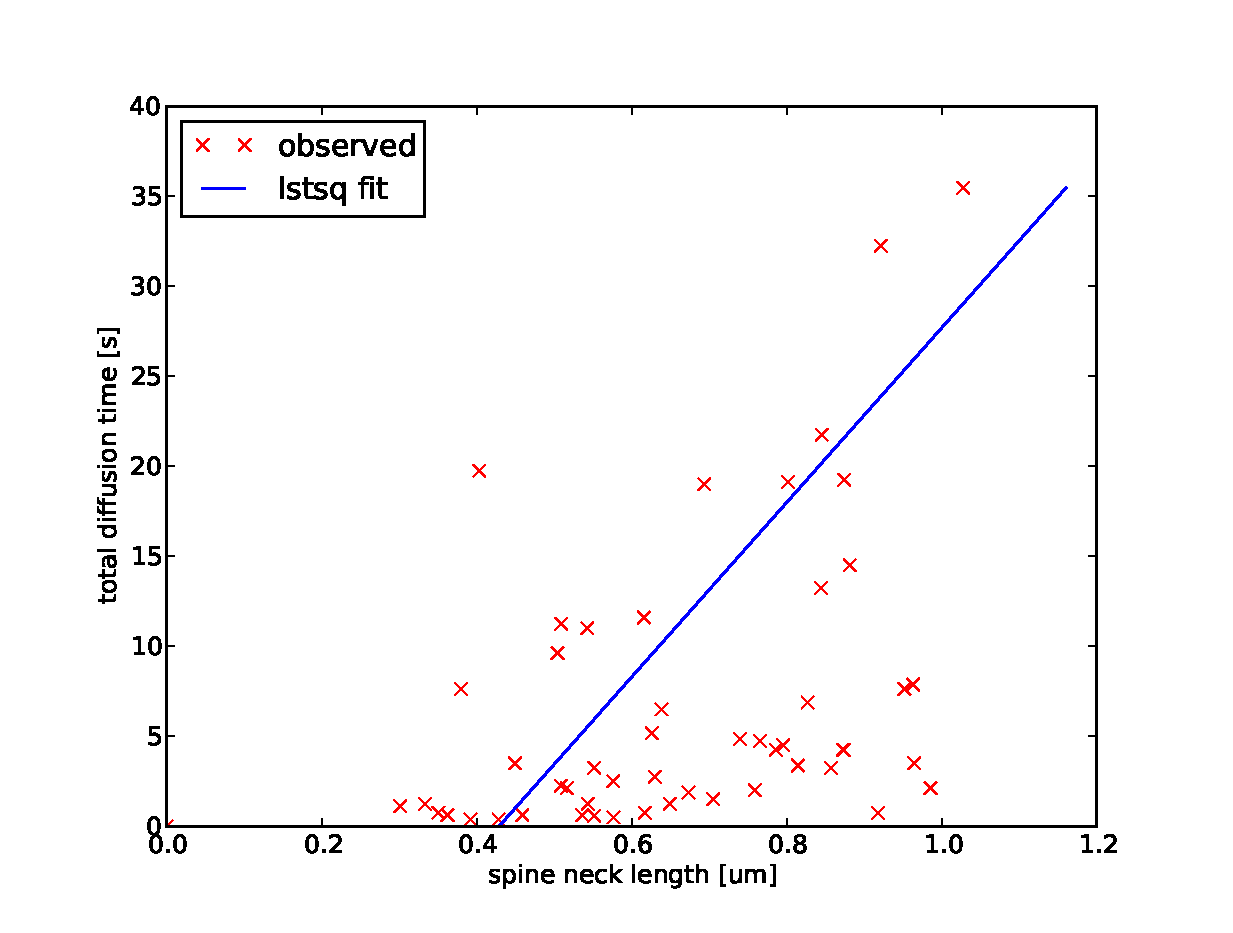
\includegraphics[width=\textwidth]{Figures/spine_stats_fulltime_nl.eps}
 \caption{Absolute diffusion times.}
 \label{results:spine_diffusion_stats:fulltime}
 \end{subfigure}
 \begin{subfigure}[b]{0.48\textwidth}
 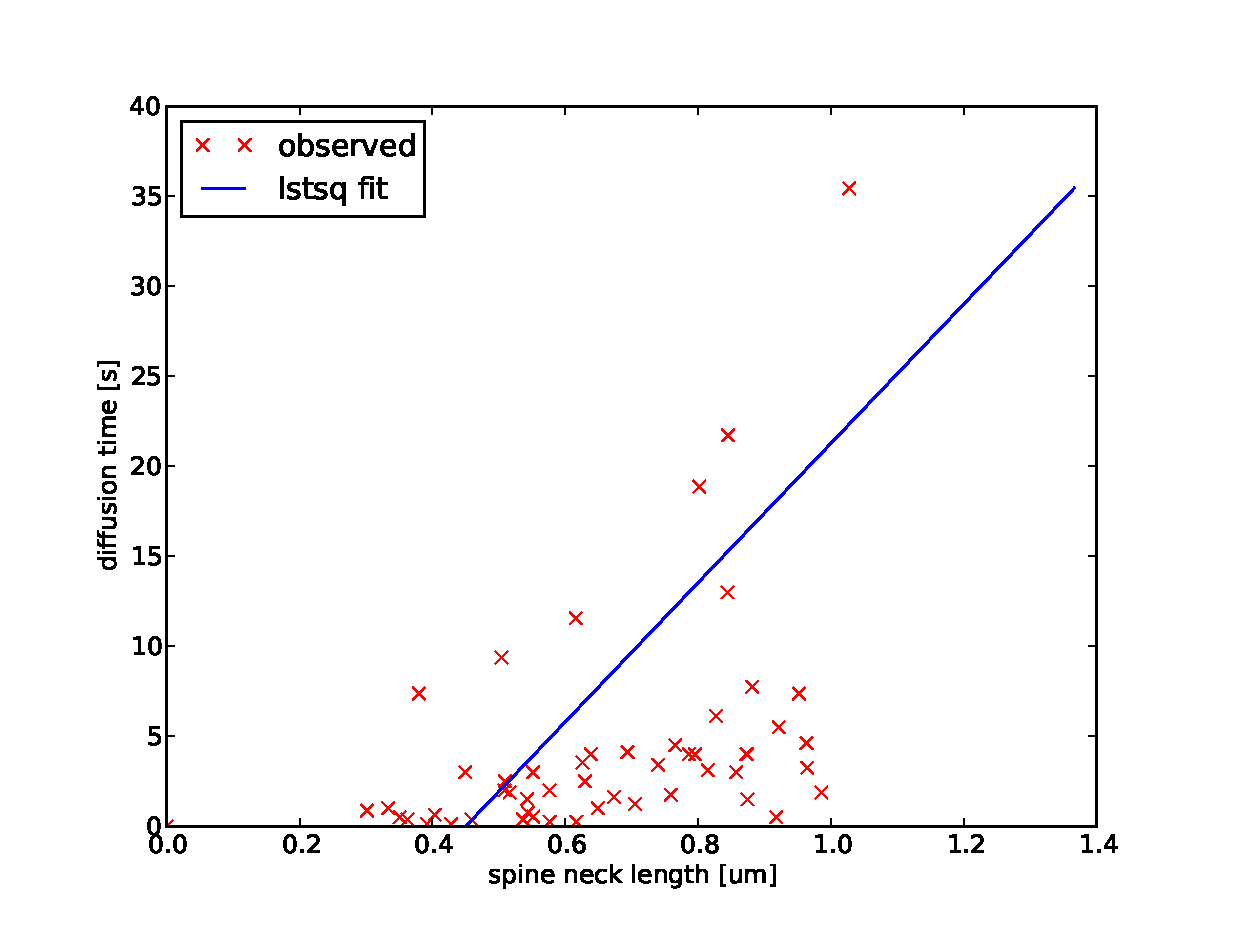
\includegraphics[width=\textwidth]{Figures/spine_stats_reltime_nl.eps}
 \caption{Relative diffusion times.}
 \label{results:spine_diffusion_stats:reltime}
\end{subfigure}
\caption[Diffusion times with least squares fit]{Absolute (a) and relative (b) diffusion times into spines. The lines represent a least squares fit of the results. This least squares fit should have been done after removing outliers and should have an expression written out somewhere.}
\label{results:spine_diffusion_stats}
\end{figure}

\begin{figure}[H]
 \centering
 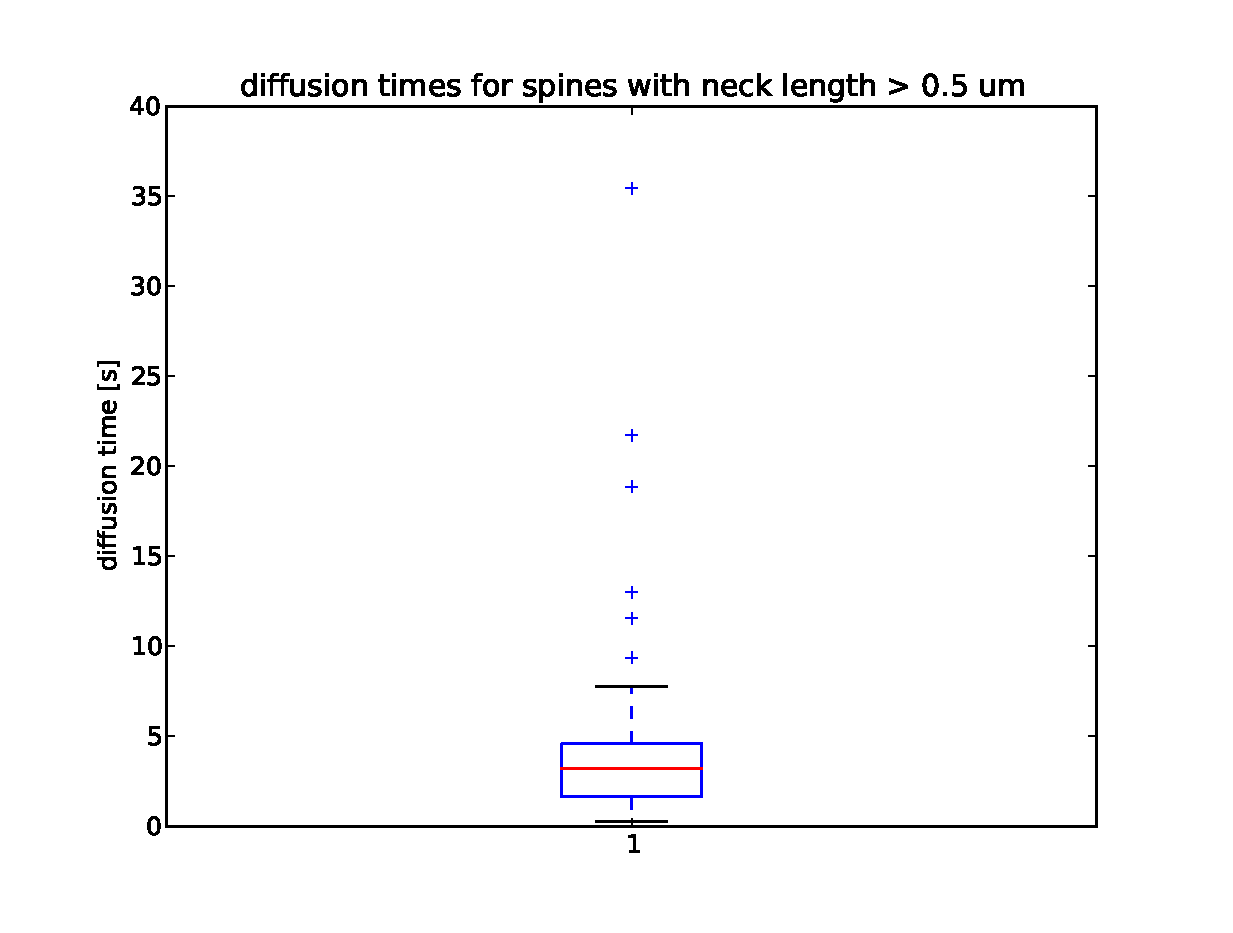
\includegraphics[scale=0.5]{Figures/spine_stats_boxplot_reltime_longneck.eps}
 \caption[Diffusion time for long necked spines]{Boxplot of the relative diffusion times (time between elevated concentration in dendrite and elevated concentration in spine head) into spines with necks longer than $0.5\mu$m. Similar studies were done by Crase et.al. and found diffusion time (unclear whether relative or not) to be somewhere around 5-10 seconds.}
 \label{results:boxplot_relative_diffusiontime_long_neck}
\end{figure}

Through the simulations it became apparent that there must be some sort of limiting factor which limits the number of PKC$\gamma$ particles that are let into the spine. 
In real life this is achieved by a concentration gradient which tends to zero (or negative values) meaning that no particles will diffuse into the spine after it is ``filled'' up. 
A random walker will not feel this concentration gradient unless it is explicitly told so. 
The alternative solution then, is to reduce the probability for particles to diffuse into a spine for each particle that get caught in the spine head by a factor $\frac{1}{10}$. 